\newpage
\subsection{Quicksearch}

Mit dem Quicksearch Algorithmus kann man ein Pattern in einer 
Zeichenfolge lokalisieren. Hierzu benötigt man einerseits das
Pattern \verb!p! und die Zeichenfolge \verb!a!.

\begin{table}[h!]
	\centering
	\begin{tabular}{l c l}
		Zeichenfolge
			& \verb!a!
			& \verb!ABADDBCCCABAACBB! \\
		Pattern
			& \verb!p!
			& \verb!ABAC! \\
	\end{tabular}
\end{table}

\noindent
Um das Pattern zu lokalisieren benötigt man ein Shiftarray \verb!s!.
Dieses muss speziell initialisert werden. Hierzu muss als erstes die 
Länge des Patterns bestimmt werden. In unserem Beispiel wäre die
Pätternlänge \verb!m! $=4$. Danach macht man ein Shiftarray, welches
so viele Elemente hat wie das Alphabet welches man benutzt. In unserem
Beispiel wären dies \verb!A,B,C,D! $=4$.

\begin{enumerate}
	\item \textbf{Initialisieren des Shiftarrays} \\
		In jedes Element des Shiftarrays \verb!s! ist der
		Wert \verb!m!$+1$ einzutragen (also 5).
		\begin{figure}[h!]
			\centering
			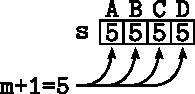
\includegraphics[scale=0.9]{quicksearch-1.pdf} 
		\end{figure}
	\item \textbf{Anpassen des Shiftarrays für vorkommende Zeichen 
		im Pattern} \\
		Das Pattern \verb!p! wird durchlaufen mit Index \verb!i!
		und \verb!m!$-$\verb!i! in das zutreffende Element vom
		Shiftarray eingetragen. Die kleine Zahl überwiegt!
		\begin{figure}[h!]
			\centering
			\hfill{} \hfill{}
			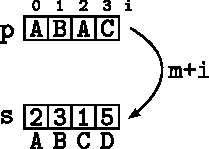
\includegraphics[scale=0.9]{quicksearch-2.pdf}
			\hfill{}
			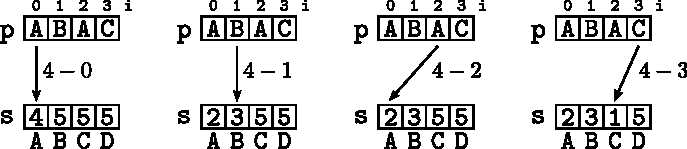
\includegraphics[scale=0.9]{quicksearch-3.pdf}
		\end{figure}
\end{enumerate}

\noindent
Nachdem das Shiftarray \verb!s! initialisert worden ist, kann mit der
Suche begonnen werden. Hierzu nimmt man das erste Zeichen des Patterns
\verb!p! und verlgeicht mit dem ersten Zeichen der Zeichenfolge \verb!a!.
Stimmt das Zeichen aus Pattern und Zeichenfolge überein, dann vergleicht
man das nächste Zeichen usw. Stimmen die Zeichen nicht überein, so
muss man in der Zeichenfolge \verb!a! vorrücken und zwar um so viele 
Stellen, wie es bis zum Ende des Pattern \verb!p! noch gibt $+1$.

\begin{figure}[h!]
	\centering
	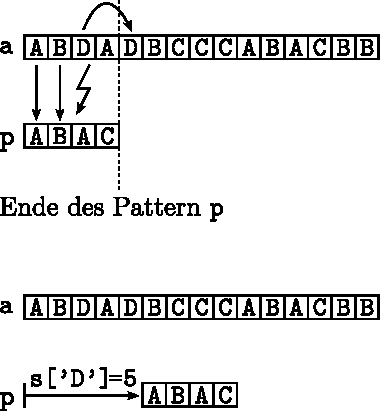
\includegraphics[scale=0.9]{quicksearch-7.pdf}
\end{figure}

\subsubsection{Implementierung}
\lstinputlisting[title=Quicksearch in Java]{quicksearch.java}



